\section{Theory} \label{sec:theory}
To calculate the energies, we need to solve the Schrödinger equation
\begin{equation}
\hat{H}\ket{\Psi_p}=\varepsilon_p\ket{\Psi_p}
\end{equation}
where we expect to find the exact ground state energy, $\varepsilon_0$, when the correct ground state wave function (GSWF) has been used. In this project we will stick to the Born-Oppenheimer approximation, which gives the Hamiltonian when the nucleus is stationary (is not affected by the electrons),
\begin{equation}
\hat{H}=\sum_{i=1}^Nt(x_i)-\sum_{i=1}^Nk\frac{Ze^2}{r_i}+\sum_{i<j}^N\frac{ke^2}{r_{ij}}.
\end{equation}
The first term gives the kinetic energy, the second gives the energy from the external potential (nucleus) and the last term gives the interaction energy. $Z$ is the atomic number, defining the number of protons in the nucleus, $k$ is the constant from Coulomb's law and $e$ is the elementary change.

We now introduce the atomic units, setting $\hbar=c=e=m_e=k=1$. 
The energies can be converted between atomic units and electronvolts using the relation
\begin{equation}
1 \text{ a.u.} = 2\cdot13.6 \text{ eV}.
\end{equation}
The Hamiltonian thus reads
\begin{equation}
\hat{H}=\hat{H}_0 + \hat{H}_I=\sum_{i=1}^N\hat{h}_0(x_i)+\sum_{i<j}^N\frac{1}{r_{ij}}
\end{equation}
with $r_{ij}\equiv\frac{1}{|\boldsymbol{r}_i-\boldsymbol{r}_j|}$ and $\hat{h}_0$ as the one-body operator for each electron. The single particle functions (SPF) are assumed to be hydrogen-like, where the one-body energies are known from the Bohr model, stating
\begin{equation}
E_n=-\frac{Z^2}{2n^2}
\end{equation}
where $n$ is the number of nodes in the wave function. In order to calculate the two-body energies, we need to solve the integrals 
\begin{equation}
\int r_1^2dr_1\int r_2^2dr_2 \Phi_{\alpha}^*(r_1)\Phi_{\beta}^*(r_2)\frac{1}{|\boldsymbol{r}_1-\boldsymbol{r}_2|}\Phi_{\gamma}(r_1)\Phi_{\delta}(r_2)\equiv\mel{\alpha\beta}{\hat{v}}{\gamma\delta}
\end{equation}
where the Dirac notation is used for shorthand notation. Note carefully that the $\Phi$'s are the total wave functions, where both the radial and spin parts are included. The spin part is known to not affect the energies, and it can therefore be factorized out,
\begin{align}
\mel{\alpha\beta}{\hat{v}}{\gamma\delta}&=(\alpha\beta|\hat{v}|\gamma\delta)\braket{\chi_{\alpha}\chi_{\beta}}{\chi_{\gamma}\chi_{\delta}}\notag\\
&=(\alpha\beta|\hat{v}|\gamma\delta)\braket{\chi_{\alpha}}{\chi_{\gamma}}\braket{\chi_{\beta}}{\chi_{\delta}}\\
&=(\alpha\beta|\hat{v}|\gamma\delta)\,\delta_{\sigma_{\alpha}\sigma_{\gamma}}\delta_{\sigma_{\beta}\sigma_{\delta}}.\notag
\end{align}
We observe that the integral is non-zero if and only if $\alpha$ and $\gamma$ got the same spin, and $\beta$ and $\delta$ got the same spin.

\subsection{Second Quantization}
For quick and compact calculations, we use second quantization as our formalism. The idea is to introduce creation and annihilation operators, which working on a Slater Determinant (SD) can create or annihilate a particle. A creation operator acting on a SD containing zero particles (called a vacuum state), will result in a SD containing one particle, and an annihilation operator acting on a SD containing zero particles will just give zero,
\begin{align}
	a_{p}^{\dagger}\ket{0}&=\ket{p}\\
	a_{p}\ket{0}&=0.
\end{align}
where $a_p^{\dagger}$ is the creation operator and $a_p$ is the annihilation operator. Note that we again use Dirac notation for the Slater Determinant. This simplifies things a lot, since we can rewrite
\begin{equation}
\begin{vmatrix}
\phi_1(x_1) & \phi_1(x_2) & \hdots & \phi_1(x_N) \\
\phi_2(x_1) & \phi_2(x_2) & \hdots & \phi_2(x_N) \\
\vdots & \vdots & \ddots &\\
\phi_N(x_1) & \phi_N(x_2) & \hdots & \phi_N(x_N)
\end{vmatrix}
\equiv \ket{1,2,\hdots,N}
\end{equation}

Further, the Slater Determinant can only contain one particle in the same state at the same time (ref. Pauli principle), such that adding a particle that already exists in the SD should automatically give zero. In the same manner, removing a particle that does not exist should also give zero. The operations that contribute are when adding a particle that does not exist and removing a particle that exists:
\begin{align}
	&a_{a}^{\dagger}\ket{abc\hdots xyz}=0\\
	&a_{a}\ket{bc\hdots xyz}=0\\
	&a_{a}^{\dagger}\ket{bc\hdots xyz}=\ket{abc\hdots xyz}\\
	&a_{a}\ket{abc\hdots xyz}=\ket{bc\hdots xyz}.
\end{align}

If we now look at a sequence of creation and annihilation operators, shuffling two operators of the same kind will just give a negative sign. On the other hand, when shuffling a creation operator with an annihilation operator, we get a Kroenecker delta minus the new ordering,
\begin{align}
	\{a_p^{\dagger},a_q^{\dagger}\}&\equiv a_p^{\dagger}a_q^{\dagger}-a_p^{\dagger}a_q^{\dagger}=0\\
	\{a_p,a_q\}&\equiv a_pa_q-a_pa_q=0\\
	\{a_p^{\dagger},a_q\}&\equiv a_p^{\dagger}a_q+a_pa_q^{\dagger}=\delta_{pq}.
\end{align}
With a sequence of operators acting on a vacuum state, we can use this to determine expectation values by moving annihilation operators against the vacuum. However, this is really tedious when we have many operators, and fortunately we have Wick's theorem to simplify these operations. More about that in section \eqref{sec:wick}.

The one-body Hamiltonian is in second quantization given by
\begin{equation}
	H_0=\frac{1}{2}\sum_{\alpha\beta}\mel{\alpha}{\hat{h}_0}{\beta}a_{\alpha}^{\dagger}a_{\beta}
\end{equation}
while the interaction part is given by
\begin{equation}
	H_I=\frac{1}{4}\sum_{\alpha\beta\gamma\delta}\mel{\alpha\beta}{\hat{v}}{\gamma\delta}_{\text{AS}}a_{\alpha}^{\dagger}a_{\beta}^{\dagger}a_{\delta}a_{\gamma}.
\end{equation}

\subsubsection{Particle-hole formalism}
For large system, it is not very tempting to write out the entire Slater Determinant as operators acting on the vacuum state. If we assume that the Slater is orthonormal onto itself, $\braket{SD}{SD}=1$, we can redefine our vacuum containing all states in the $\ket{SD}$. This is often called the Fermi vacuum. When annihilating a particle below the Fermi level (one of the particles in the Fermi vacuum), we say that we create a hole. When replacing the hole with a particle, we say that we annihilate the hole. Similarly above the Fermi level, we can create and annihilate particles. The annihilation operator therefore now works as before above the Fermi level, but below the Fermi level the creation operator works as the annihilation operator before, and vice versa. In that manner, we specify whether the quasiparticle is a hole or a particle by giving holes indices $i,j,k,l,\hdots$ and particles indices $a,b,c,d,\hdots$. $p,q,r,s,\hdots$ are without restrictions. This leads to
\begin{align}
	\{a_a^{\dagger},a_b\}&=\delta_{ab}\\
	\{a_i,a_j^{\dagger}\}&=\delta_{ij}
\end{align}
which we again can use to calculate expectation values, or just to simplify. 

\subsubsection{Wick's theorem} \label{sec:wick}
Wick's theorem is extremely useful when calculating expectation values in second quantization. It states that a sequence of operators can be written as the normal ordering of the operators plus the sum over all normal orderings after one contraction plus the sum over all normal orderings after two contractions and so on and so forth. Mathematically, we can write it as
\begin{align}
	ABC\hdots XYZ=&\{ABC\hdots XYZ\}\\
	&+\sum_{\text{Single cont.}}\{\wick{AB \c1C\hdots \c1XYZ}\}\\
	&+\sum_{\text{Double cont.}}\{\wick{A \c2B \c1C\hdots \c1X \c2YZ}\}\\
	&+\hdots
\end{align}

Immediately, it does not seem to simplify the sequence, the clue lies in the normalizing. When calculating expectation values, we will always have an equal number of creation and annihilation operators between the vacuum states (otherwise the expectation value is zero). This means that a normal ordering will always contain an annihilation operator, which is located to the right, acts on the vacuum state and everything goes to zero. In other words, the only terms that contribute in an expectation value calculation are the fully contracted terms, which gives a major simplification. 

The theorem can also be generalized, taking operators of multiple creation and annihilation operators into account. If those operators are normal ordered, Wick's theorem states that only external contractions will contribute, i.e, no contractions inward the operators. [https://manybodyphysics.github.io/FYS4480/doc/pub/secondquant/html/secondquant-bs.html]

\subsubsection{Energy formulas}
We are now ready to calculate some expectation values based on the theory above. We will later do Configuration Interaction Singles (CIS) only, so it is sufficient to calculate $\mel{\Phi_0}{\hat{H}}{\Phi_0}$, $\mel{\Phi_0}{\hat{H}}{\Phi_i^a}$ and $\mel{\Phi_i^a}{\hat{H}}{\Phi_j^b}$. The calculations are moved to Appendix A in order to maintain some sort of neatness. We obtain that the reference energy as a function
of $Z$ is
\begin{align}
	\varepsilon_0=\mel{\Phi_0}{\hat{H}}{\Phi_0}&=\sum_i\mel{i}{\hat{h}_0}{i}+\frac{1}{2}\sum_{ij}\mel{ij}{\hat{v}}{ij}_{\text{AS}}\label{eq:c_H_c}
\end{align}
where the subscript AS indicates an antisymmetric elements,
\begin{equation}
\mel{ij}{\hat{v}}{ij}_{\text{AS}}=\mel{ij}{\hat{v}}{ij}-\mel{ij}{\hat{v}}{ji}.
\end{equation}
Further, we obtained
\begin{equation}
\mel{\Phi_0}{\hat{H}}{\Phi_i^a}=\mel{i}{\hat{h}_0}{a}+\sum_j\mel{aj}{\hat{v}}{ij}_{\text{AS}}
\label{eq:c_H_ia}
\end{equation}
and
\begin{align}
	\mel{\Phi_i^a}{\hat{H}}{\Phi_j^b}=\mel{aj}{\hat{v}}{ib}_{\text{AS}}&-\delta_{ab}\Big[\mel{i}{\hat{h}_0}{j}+\sum_k\mel{ik}{\hat{v}}{jk}_{\text{AS}}\Big]\notag\\
	&+\delta_{ij}\Big[\mel{a}{\hat{h}_0}{b}+\sum_k\mel{ak}{\hat{v}}{bk}_{\text{AS}}\Big]\\
	&+\delta_{ab}\delta_{ij}\Big[\sum_k\mel{k}{\hat{h}_0}{k}+\frac{1}{2}\sum_{kl}\mel{kl}{\hat{v}}{kl}_{\text{AS}}\Big]\notag
	\label{eq:ia_H_jb}
\end{align}
where the two latter are functions of $Z$ as well. They are then general.

\subsection{The Helium atom}
A neutral Helium atom consists of a nucleus of two protons with two electrons orbiting, and is the simplest many-body atom one can study (atoms with more than 1 electron). The difficulty of dealing with many-body systems lies in the interaction, where the elements $\mel{\alpha\beta}{\hat{v}}{\gamma\delta}$ can be really tricky to handle. The interaction term makes the exact wave function almost impossible to find.

There exist various methods for solving this problem, where one of the most successful is to define a wave function which is varied such that the energy is minimized. This method was used by E. Hylleraas already in 1929, when he minimized the energy with a wave function of 10 variational parameters, using a mechanical desk calculator. [https://www.encyclopedia.com/science/dictionaries-thesauruses-pictures-and-press-releases/hylleraas-egil-andersen] He found the energy to be -2.90363 eV, which is close to recent experimental values, and which we will compare our energies to.  [http://www.umich.edu/~chem461/QMChap8.pdf][https://journals.aps.org/prl/abstract/10.1103/PhysRevLett.80.3475]. 

\subsubsection{Ground state}
Helium is in its ground state when both electrons occupy the 1s orbital, thus they have opposite spins and $M_s=0$. In this project, we will study systems of $M_s=0$ only, such that an electron can only be excited to a state with the same spin. 

Taking the Pauli principle into account, the two-body wavefunction needs to be nulled out if two particles are in the same state, and it should also be antisymmetric under exchange of two particles. We are therefore in need of a Slater Determinant, given by
\begin{align}
	\Psi(x_1,x_2,\sigma_1,\sigma_2)&=A\mqty|\psi_{\sigma_1}(x_1) & \psi_{\sigma_1}(x_2)\\ \psi_{\sigma_2}(x_1) & \psi_{\sigma_2}(x_2)|\\
	&=A\Big[\psi_{\sigma_1}(x_1)\psi_{\sigma_2}(x_2)-\psi_{\sigma_2}(x_1)\psi_{\sigma_1}(x_2)\Big]
\end{align}
where $\psi_{\sigma_1}$ is the SPF with spin $m_s=\sigma_1$ and $A$ is a normalization constant. If we assume that the SPFs are normalized, our ansatz can be written as
\begin{equation}
\ket{\Phi_0}=\frac{1}{\sqrt{2}}(\ket{1}\ket{\bar{1}}-\ket{\bar{1}}\ket{1})
\end{equation}
with $\ket{\bar{1}}$ describing a particle with principle quantum number 1 and spin $\sigma_2$, which we will illustrate with spin down. In second quantization, we can construct the ground state from the true vacuum,
\begin{equation}
\ket{\Phi_0}=a_{1}^{\dagger}a_{\bar{1}}^{\dagger}\ket{0},
\end{equation}
which is understand to take the anti-symmetry property. The ground state is illustrated in figure \eqref{fig:schematic_he_gs}.
\begin{figure} [H]
	\begin{center}
		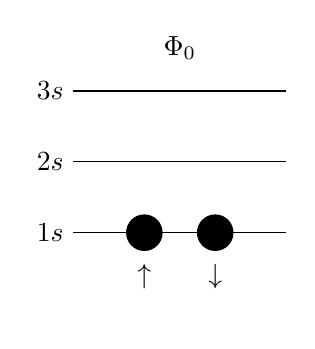
\begin{tikzpicture}[scale=0.9]
		\begin{scope}
			\foreach \i in {1,...,3}
			{
				\draw (-1,\i-1) node[anchor=east] {$\i s$} --(2,\i-1);
			}
			\filldraw (0,0) node[anchor=north,inner sep=.4cm] {$\uparrow$} circle (0.25cm); 
			\filldraw (1,0) node[anchor=north,inner sep=.4cm] {$\downarrow$} circle (0.25cm);
			\node[] at (0.5,2.6) {$\ket{\Phi_0}$};
		\end{scope}
		\end{tikzpicture}
	\end{center}
\caption{Ground state of Helium.}
\label{fig:schematic_he_gs}
\end{figure}

\subsubsection{Excited states}
When entering excited states, we can risk having angular quantum numbers unlike zero, because $l\in[0,n-1]$. This makes the computations more difficult, but in this project we will ignore that challenge setting $l=0$, and thus limit us to the s-waves. 

Consider now a system consisting of the orbitals 1s, 2s and 3s only. For that case, the possible energy states of the Helium atom are listed in figure \eqref{fig:schematic_he}.
\begin{figure} [H]
	\begin{center}
		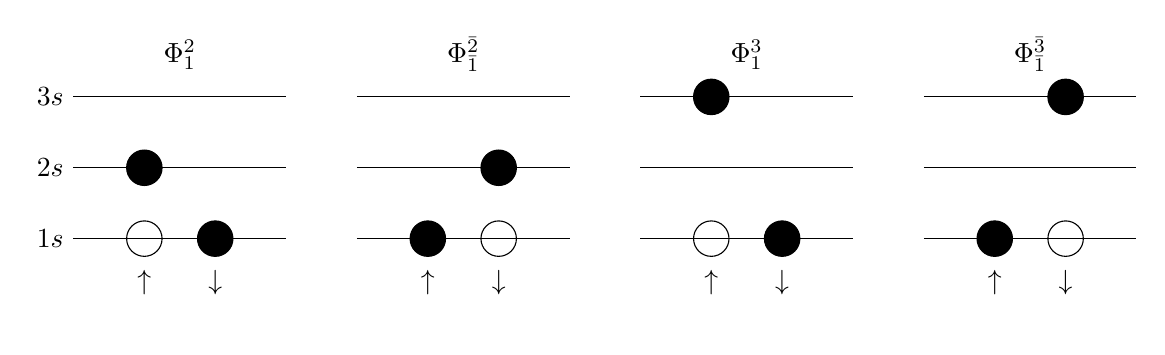
\begin{tikzpicture}[scale=0.9]
		\begin{scope}
		\foreach \i in {1,...,3}
		{
			\draw (-1,\i-1) node[anchor=east] {$\i s$} --(2,\i-1);
		}
		\draw (0,0) node[anchor=north,inner sep=.4cm] {$\uparrow$} circle (0.25cm); 
		\filldraw (1,0) node[anchor=north,inner sep=.4cm] {$\downarrow$} circle (0.25cm);
		\filldraw (0,1) circle (0.25cm);
		\node[] at (0.5,2.6) {$\ket{\Phi_{1}^{2}}$};
		\end{scope}
		\begin{scope}[xshift=4cm]
		\foreach \i in {1,...,3}
		{
			\draw (-1,\i-1) --(2,\i-1);
		}
		\filldraw (0,0) node[anchor=north,inner sep=.4cm] {$\uparrow$} circle (0.25cm); 
		\draw (1,0) node[anchor=north,inner sep=.4cm] {$\downarrow$} circle (0.25cm);
		\filldraw (1,1) circle (0.25cm);
		\node[] at (0.5,2.6) {$\ket{\Phi_{\bar{1}}^{\bar{2}}}$};
		\end{scope}
		\begin{scope}[xshift=8cm]
		\foreach \i in {1,...,3}
		{
			\draw (-1,\i-1) --(2,\i-1);
		}
		\draw (0,0) node[anchor=north,inner sep=.4cm] {$\uparrow$} circle (0.25cm); 
		\filldraw (1,0) node[anchor=north,inner sep=.4cm] {$\downarrow$} circle (0.25cm);
		\filldraw (0,2) circle (0.25cm); 
		\node[] at (0.5,2.6) {$\ket{\Phi_{1}^{3}}$};
		\end{scope}
		\begin{scope}[xshift=12cm]
		\foreach \i in {1,...,3}
		{
			\draw (-1,\i-1) --(2,\i-1);
		}
		\filldraw (0,0) node[anchor=north,inner sep=.4cm] {$\uparrow$} circle (0.25cm); 
		\draw (1,0) node[anchor=north,inner sep=.4cm] {$\downarrow$} circle (0.25cm);
		\filldraw (1,2) circle (0.25cm); 
		\node[] at (0.5,2.6) {$\ket{\Phi_{\bar{1}}^{\bar{3}}}$};
		\end{scope}
		\end{tikzpicture}
		\newline
		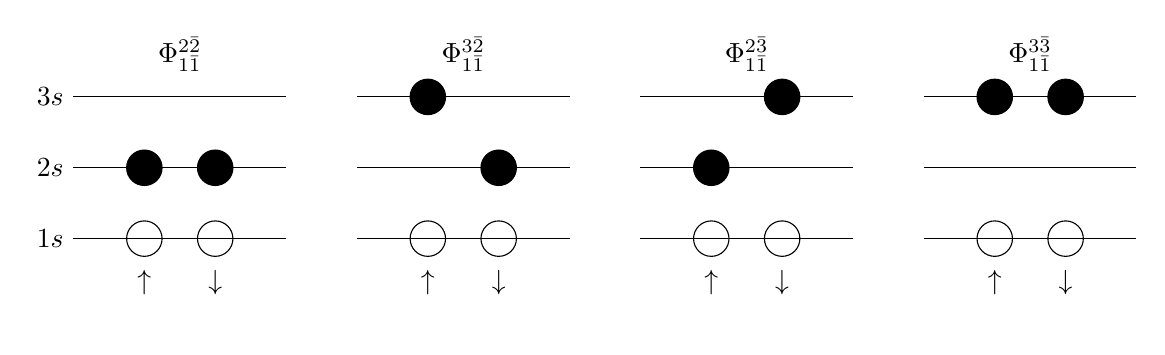
\begin{tikzpicture}[scale=0.9]
		\begin{scope}
		\foreach \i in {1,...,3}
		{
			\draw (-1,\i-1) node[anchor=east] {$\i s$} --(2,\i-1);
		}
		\draw (0,0) node[anchor=north,inner sep=.4cm] {$\uparrow$} circle (0.25cm); 
		\draw (1,0) node[anchor=north,inner sep=.4cm] {$\downarrow$} circle (0.25cm);
		\filldraw (0,1) circle (0.25cm);
		\filldraw (1,1) circle (0.25cm);
		\node[] at (0.5,2.6) {$\ket{\Phi_{1\bar{1}}^{2\bar{2}}}$};
		\end{scope}
		\begin{scope}[xshift=4cm]
		\foreach \i in {1,...,3}
		{
			\draw (-1,\i-1) --(2,\i-1);
		}
		\draw (0,0) node[anchor=north,inner sep=.4cm] {$\uparrow$} circle (0.25cm); 
		\draw (1,0) node[anchor=north,inner sep=.4cm] {$\downarrow$} circle (0.25cm);
		\filldraw (0,2) circle (0.25cm); 
		\filldraw (1,1) circle (0.25cm); 
		\node[] at (0.5,2.6) {$\ket{\Phi_{1\bar{1}}^{3\bar{2}}}$};
		\end{scope}
		\begin{scope}[xshift=8cm]
		\foreach \i in {1,...,3}
		{
			\draw (-1,\i-1) --(2,\i-1);
		}
		\draw (0,0) node[anchor=north,inner sep=.4cm] {$\uparrow$} circle (0.25cm); 
		\draw (1,0) node[anchor=north,inner sep=.4cm] {$\downarrow$} circle (0.25cm);
		\filldraw (1,2) circle (0.25cm);
		\filldraw (0,1) circle (0.25cm);
		\node[] at (0.5,2.6) {$\ket{\Phi_{1\bar{1}}^{2\bar{3}}}$};
		\end{scope}
		\begin{scope}[xshift=12cm]
		\foreach \i in {1,...,3}
		{
			\draw (-1,\i-1) --(2,\i-1);
		}
		\draw (0,0) node[anchor=north,inner sep=.4cm] {$\uparrow$} circle (0.25cm); 
		\draw (1,0) node[anchor=north,inner sep=.4cm] {$\downarrow$} circle (0.25cm);
		\filldraw (0,2) circle (0.25cm); 
		\filldraw (1,2) circle (0.25cm);
		\node[] at (0.5,2.6) {$\ket{\Phi_{1\bar{1}}^{3\bar{3}}}$};
		\end{scope}
		\end{tikzpicture}
	\end{center}
	\caption{Possible states in the 1s, 2s and 3s orbitals of Helium. In the first row, all singly excited states are listed, while in the second row all doubly excited states are listed.}
	\label{fig:schematic_he}
\end{figure}

\subsection{The Beryllium atom}
Beryllium has atomic number $Z=4$, so a neutral Beryllium atom has four protons in its nucleus and four electrons swarming around. To study atoms with even atomic numbers is easier than odd atomic number, since the Fermi level is well defined. 

\subsubsection{Ground state}
Beryllium is in its ground state when the electrons occupy the 1s and 2s orbitals (we again set $l=0$). In second quantization, the ground state can then be expressed as
\begin{equation}
\ket{\Phi_0}=a_{1}^{\dagger}a_{\bar{1}}^{\dagger}a_{2}^{\dagger}a_{\bar{2}}^{\dagger}\ket{0},
\end{equation}
and is illustrated in figure \eqref{fig:schematic_be_gs}.
\begin{figure} [H]
	\begin{center}
		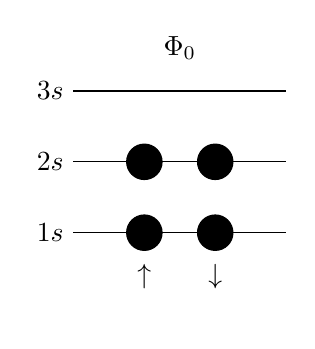
\begin{tikzpicture}[scale=0.9]
		\begin{scope}
		\foreach \i in {1,...,3}
		{
			\draw (-1,\i-1) node[anchor=east] {$\i s$} --(2,\i-1);
		}
		\filldraw (0,0) node[anchor=north,inner sep=.4cm] {$\uparrow$} circle (0.25cm); 
		\filldraw (1,0) node[anchor=north,inner sep=.4cm] {$\downarrow$} circle (0.25cm);
		\filldraw (0,1) circle (0.25cm);
		\filldraw (1,1) circle (0.25cm);
		\node[] at (0.5,2.6) {$\ket{\Phi_0}$};
		\end{scope}
		\end{tikzpicture}
	\end{center}
	\caption{Ground state of Beryllium.}
	\label{fig:schematic_be_gs}
\end{figure}

\subsubsection{Excited states}
We again limit us to the 1s, 2s and 3s orbits. When the electrons have only two free slots to be excited to. Anyway, since we have four particles that can be excited, there are still as many possible excited states as for Helium, see figure \eqref{fig:schematic}.
\begin{figure} [H]
	\begin{center}
		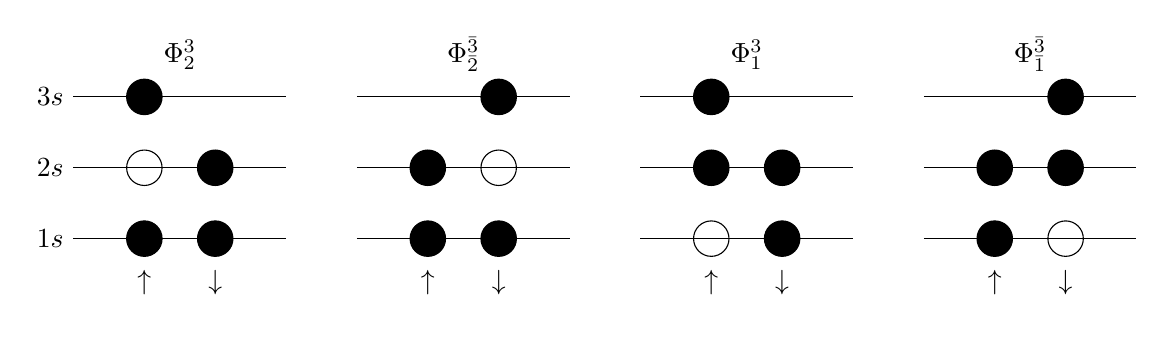
\begin{tikzpicture}[scale=0.9]
		\begin{scope}
		\foreach \i in {1,...,3}
		{
			\draw (-1,\i-1) node[anchor=east] {$\i s$} --(2,\i-1);
		}
		\filldraw (0,0) node[anchor=north,inner sep=.4cm] {$\uparrow$} circle (0.25cm); 
		\filldraw (1,0) node[anchor=north,inner sep=.4cm] {$\downarrow$} circle (0.25cm);
		\draw (0,1) circle (0.25cm);
		\filldraw (1,1) circle (0.25cm);
		\filldraw (0,2) circle (0.25cm);
		\node[] at (0.5,2.6) {$\ket{\Phi_2^3}$};
		\end{scope}
		\begin{scope}[xshift=4cm]
		\foreach \i in {1,...,3}
		{
			\draw (-1,\i-1) --(2,\i-1);
		}
		\filldraw (0,0) node[anchor=north,inner sep=.4cm] {$\uparrow$} circle (0.25cm); 
		\filldraw (1,0) node[anchor=north,inner sep=.4cm] {$\downarrow$} circle (0.25cm);
		\draw (1,1) circle (0.25cm);
		\filldraw (1,2) circle (0.25cm);
		\filldraw (0,1) circle (0.25cm);
		\node[] at (0.5,2.6) {$\ket{\Phi_{\bar{2}}^{\bar{3}}}$};
		\end{scope}
		\begin{scope}[xshift=8cm]
		\foreach \i in {1,...,3}
		{
			\draw (-1,\i-1) -- (2,\i-1);
		}
		\draw (0,0) node[anchor=north,inner sep=.4cm] {$\uparrow$} circle (0.25cm); 
		\filldraw (1,0) node[anchor=north,inner sep=.4cm] {$\downarrow$} circle (0.25cm);
		\filldraw (0,1) circle (0.25cm);
		\filldraw (1,1) circle (0.25cm);
		\filldraw (0,2) circle (0.25cm);
		\node[] at (0.5,2.6) {$\ket{\Phi_{1}^{3}}$};
		\end{scope}
		\begin{scope}[xshift=12cm]
		\foreach \i in {1,...,3}
		{
			\draw (-1,\i-1) --(2,\i-1);
		}
		\filldraw (0,0) node[anchor=north,inner sep=.4cm] {$\uparrow$} circle (0.25cm); 
		\draw (1,0) node[anchor=north,inner sep=.4cm] {$\downarrow$} circle (0.25cm);
		\filldraw (1,1) circle (0.25cm);
		\filldraw (1,2) circle (0.25cm);
		\filldraw (0,1) circle (0.25cm);
		\node[] at (0.5,2.6) {$\ket{\Phi_{\bar{1}}^{\bar{3}}}$};
		\end{scope}
		\end{tikzpicture}
		\newline
		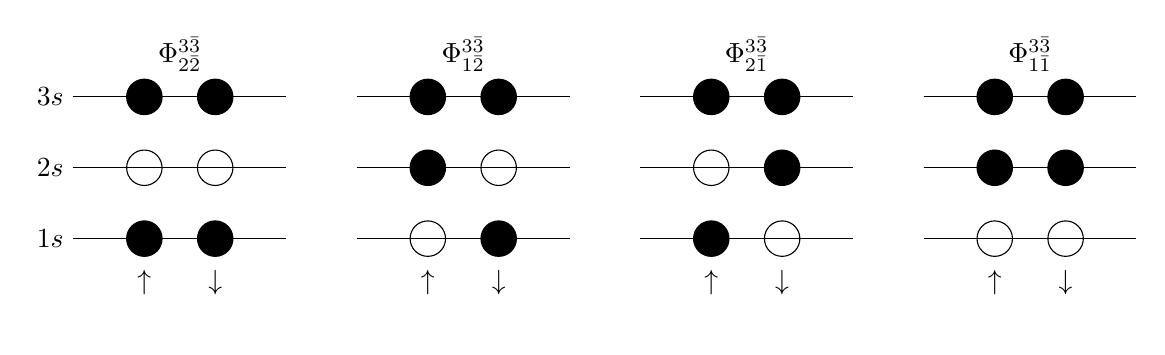
\begin{tikzpicture}[scale=0.9]
		\begin{scope}
		\foreach \i in {1,...,3}
		{
			\draw (-1,\i-1) node[anchor=east] {$\i s$} --(2,\i-1);
		}
		\filldraw (0,0) node[anchor=north,inner sep=.4cm] {$\uparrow$} circle (0.25cm); 
		\filldraw (1,0) node[anchor=north,inner sep=.4cm] {$\downarrow$} circle (0.25cm);
		\draw (0,1) circle (0.25cm);
		\draw (1,1) circle (0.25cm);
		\filldraw (0,2) circle (0.25cm);
		\filldraw (1,2) circle (0.25cm);
		\node[] at (0.5,2.6) {$\ket{\Phi_{2\bar{2}}^{3\bar{3}}}$};
		\end{scope}
		\begin{scope}[xshift=4cm]
		\foreach \i in {1,...,3}
		{
			\draw (-1,\i-1) --(2,\i-1);
		}
		\draw (0,0) node[anchor=north,inner sep=.4cm] {$\uparrow$} circle (0.25cm); 
		\filldraw (1,0) node[anchor=north,inner sep=.4cm] {$\downarrow$} circle (0.25cm);
		\draw (1,1) circle (0.25cm);
		\filldraw (1,2) circle (0.25cm);
		\filldraw (0,2) circle (0.25cm);
		\filldraw (0,1) circle (0.25cm);
		\node[] at (0.5,2.6) {$\ket{\Phi_{1\bar{2}}^{3\bar{3}}}$};
		\end{scope}
		\begin{scope}[xshift=8cm]
		\foreach \i in {1,...,3}
		{
			\draw (-1,\i-1) -- (2,\i-1);
		}
		\filldraw (0,0) node[anchor=north,inner sep=.4cm] {$\uparrow$} circle (0.25cm); 
		\draw (1,0) node[anchor=north,inner sep=.4cm] {$\downarrow$} circle (0.25cm);
		\draw (0,1) circle (0.25cm);
		\filldraw (1,1) circle (0.25cm);
		\filldraw (0,2) circle (0.25cm);
		\filldraw (1,2) circle (0.25cm);
		\node[] at (0.5,2.6) {$\ket{\Phi_{2\bar{1}}^{3\bar{3}}}$};
		\end{scope}
		\begin{scope}[xshift=12cm]
		\foreach \i in {1,...,3}
		{
			\draw (-1,\i-1) --(2,\i-1);
		}
		\draw (0,0) node[anchor=north,inner sep=.4cm] {$\uparrow$} circle (0.25cm); 
		\draw (1,0) node[anchor=north,inner sep=.4cm] {$\downarrow$} circle (0.25cm);
		\filldraw (1,1) circle (0.25cm);
		\filldraw (1,2) circle (0.25cm);
		\filldraw (0,1) circle (0.25cm);
		\filldraw (0,2) circle (0.25cm);
		\node[] at (0.5,2.6) {$\ket{\Phi_{1\bar{1}}^{3\bar{3}}}$};
		\end{scope}
		\end{tikzpicture}
	\end{center}
	\caption{Possible states in the 1s, 2s and 3s orbitals of Beryllium. In the first row, all singly excited states are listed, while in the second row all doubly excited states are listed.}
	\label{fig:schematic}
\end{figure}